\chapter{Ben Farr, Winter 2025}
\section{Newtonian gravity}
The newtonian formula for gravitational attraction is $F = \frac{Gm_1 m_2}{r_{12}^2}$. This formula unfortunately doesn't agree with special relativity, in that the attractive force has no speed of light propogation.
Although the shift to general relativity will change this a bit, a few things still persist. Gravity is not screened by opposing charges, and it is extremely long range in both the newtonian and einsteinian description.

Comparing the relative forces between different fundamental forces we can take a pair of protons as our example:
\begin{align*}
	\frac{F_\text{grav}}{F_{EM}} &= \frac{Gm_p^2}{\frac{e^2}{4\pi\epsilon_0}} \\
	\frac{F_\text{grav}}{F_{EM}} &~ 10^{-36}
\end{align*}
This of course doesn't drive the motion of the universe as most charges end up screened on large scales.

Looking instead at the importance of using the generally relativistic formulation instead of the newtonian description we have another quantity we want to consider. The quantity $\frac{GM}{Rc^2}$ will describe the relative importance for gerneral relativity.
If we look at earth, we see a value of $10^{-9}$, which is only important for extremely precise measurements. For the sun we see $10^{-6}$, which ended up primarily showing up in the perihilion precession of mercury.
For Neutron stars we see a value of $0.1$. And finally looking at black holes we see at the event horizon $0.5$. Due to coincidence (potentially) it turns out we can calculate the excape velocity using newtonian mechanics.

\begin{figure*}[h]
	\centering
	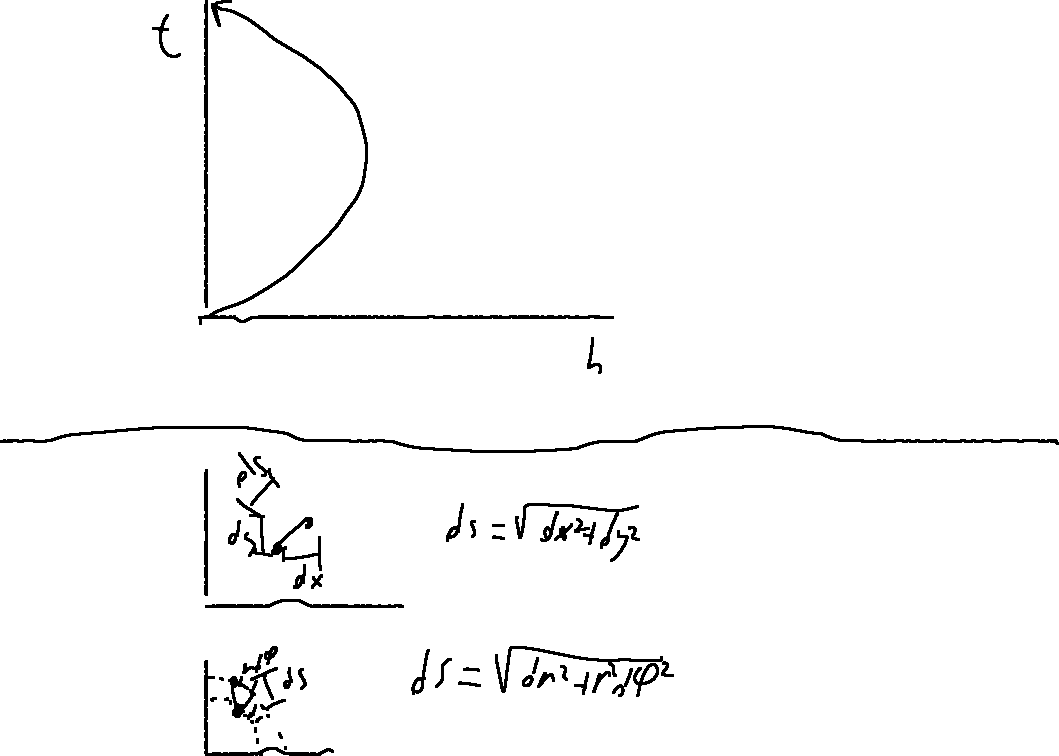
\includegraphics[width=10cm]{1-07-1.png}
	\caption*{Euclidean Geometries}
\end{figure*}
If we now seek to calculate the circumference of a circle using these two different coordinate systems:
\begin{align*}
	C &= \int ds \\
	C &= \int \sqrt{dx^2 + dy^2} \\
	C &= 2\int_-R^R \sqrt{1 + y'\ ^2}dx \\
	C &= 2R\int_-1^1 \frac{dv}{\sqrt{1-v^2}} \\
	C &= 2\pi R
\end{align*}
In the case of polar coordinates though:
\begin{align*}
	C &= \int ds \\
	C &= \int_0^{2\pi} R d\phi \\
	C &= 2\pi R
\end{align*}

We can see that both of these describe Euclidean geometries, but if we move to the Geometry on the surface of a sphere:

The line element is:
\begin{align*}
	ds^2 &= a^2 d\theta^2 + a^2\sin^2\theta d\phi^2
\end{align*}
We can w.l.o.g rotate our sphere such that our circle is moving along a curve where $\theta$ is constant. Therefore we have:
\begin{align*}
	ds &= a\sin\theta d\phi \\
	C &= a2\pi \sin\theta
\end{align*}
If instead we have a circle of radius r, on a sphere of radius a, we choose coordinates with varying $\theta$ but constant $\phi$, so:
\begin{align*}
	ds &= ad\theta \\
	r &= \int ds \\
	r &= \int _0^\theta ad\theta \\
	r &= a\theta \\
	C &= 2\pi a \sin \frac{r}{a}
\end{align*}
Which matches Euclidean geometry in the small r limit.

In GR we will often take a line element and try to use it to understand the underlying geometry. For example we consider $ds^2 = a^2(d\theta^2 f^2(\theta) d\phi^2)$. If we choose $\theta = \sin\theta$ then we are working on the surface of a sphere.
The first property we can not is that the line element is unchanged with $\phi$, so this must have a symetry around the z axis. If we look at $f(\theta) = \sin\theta(1-\frac{3}{4}\sin^2\theta)$, we end up with a peanut geometry.
\begin{figure*}[h]
	\centering
	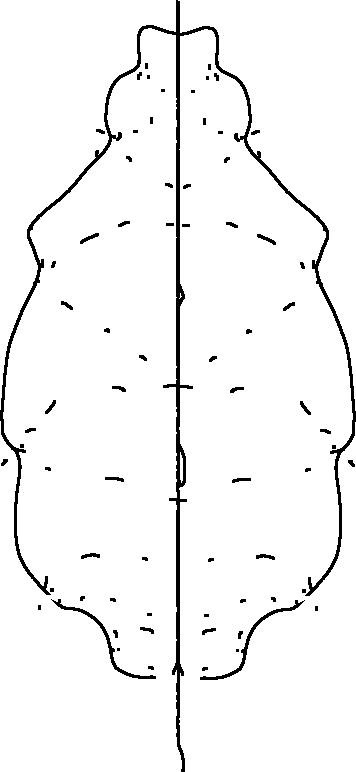
\includegraphics[width=4cm]{1-07-2.png}
	\caption*{Our general $f(\theta)$ geometry}
\end{figure*}

In an inertial frame an observer will have a set of coordinates $t$ such that $\frac{d^2x_i}{dt^2}=0$. A pair of inertial frames can differ by constant displacements, uniform velocities, and constant rotations.

Looking at a pair of frames that only differ by displacements $(x,y,z)$, $(x',y',z')$, if we have this displacement be $d$ along the x axis we know:
\begin{align*}
	x' &= x-d & y'&= y & z' &= z
\end{align*}
Instead for a rotation $\theta$ about the z axis:
\begin{align*}
	x' &= \sin\theta y + \cos\theta x &
	y' &= \cos\theta y - \sin \theta x &
	z' &= z
\end{align*}
If we inestead have a uniform velocity about the x axis, we instead have:
\begin{align*}
	x' &= x -vt' &
	y' &= y &
	z' &= z
\end{align*}

For a point mass experience a gravitational attraction we see:
\begin{align*}
	\bm{F} &= -\frac{GmM}{r^2} \hat{e}_r \\
	\Phi(\bm{x}) &= -\frac{GM}{r} \\
	\Phi(\bm{x}) &= -\frac{GM}{|\bm{x} - \bm{x}_A|}
\end{align*}
If we add multiple point masses:
\begin{align*}
	\Phi(\bm{x}) &= \sum_A-\frac{GM_A}{|\bm{x} - \bm{x}_A|}
\end{align*}
Taking the continuum limit:
\begin{align*}
	\Phi(\bm{x}) &= -\int d^3x' \frac{G\mu(\bm{x}')}{|\bm{x} - \bm{x}'|}
\end{align*}
Which gives rise to the gravitational field:
\begin{align*}
	\bm{g}(\bm{x}) &= -\del\Phi(\bm{x})
\end{align*}
From which we can take a differential form of our potential:
\begin{align*}
	\del\cdot\bm{g} &= -4\pi G\mu(\bm{x}) \\
	\del^2\Phi(\bm{x}) &= -4\pi G\mu(\bm{x}) \\
	m\bm{a} &= -m\del\Phi \\
	\bm{a} &= -\del\Phi
\end{align*}
Where we note that in Newtonian gravity the fact that gravitational mass and the inertial mass being equivalent seems to be a coincidence.
